\chapter{Lo standard MIDI}
\label{chap:midi}

\section{Il protocollo di comunicazione e i messaggi MIDI}
Nel protocollo MIDI le informazioni e gli eventi vengono trasmessi sotto forma di \textit{messaggi}.
Ogni messaggio è composto da una sequenza di byte ordinata, di cui il primo è detto \textit{status byte} e i successivi
vengono detti \textit{data byte}.
Per riconoscere gli status byte dai data byte si impone che il bit più significativo degli status byte sia sempre 1, mentre quello dei data byte sia 0,
mentre i rimanenti 7 bit possono rappresentare valori da da 0 a 127.
I primi 4 bit dello status byte identificano il tipo di messaggio MIDI, mentre gli ultimi 4 specificano il canale su cui il messaggio ha effetto,
per un massimo possibile di 16 canali.

\begin{figure}
    \centering
    \def\svgwidth{\columnwidth}
    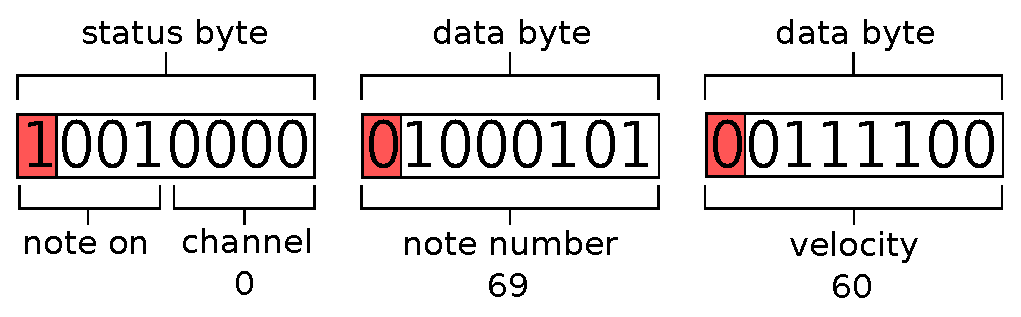
\includegraphics[width=0.7\columnwidth]{TeX_files/midi_message.eps}
    \caption{Struttura di un messaggio MIDI di tipo \textit{note on},
    	     con note number 69 e velocity 60. In rosso è evidenziato
             il bit più significativo.}
\end{figure}

Ai fini del progetto, verranno gestiti solamente i messaggi di \textbf{note on} e \textbf{note off} sul canale '0', mentre
ogni altro tipo di messaggio sarà ignorato.
Ogni messaggio di \textit{note on} viene trasmesso nel momento in cui una certa nota deve essere suonata e contiene due data byte: 
il primo, il \textbf{note number}, identifica la nota da riprodurre, mentre il secondo, detto \textbf{velocity}, fornisce un'informazione
sull'intensità con cui la nota viene suonata. Il suo status byte è del tipo
\textit{1001xxxx} dove \textit{xxxx} sta ad indicare il canale del
messaggio.
Il messaggio note off è analogo e viene trasmesso quando si vuole
interrompere la riproduzione di una certa nota, e il suo status byte
ha il formato \textit{1000xxxx}.
Un altro modo di interrompere la nota (citare standard) è quello di mandare
un messaggio \textit{note on} con \textit{velocity} impostata a zero.

\section{Physical Layer}
I messaggi MIDI vengono trasmessi in maniera seriale e vengono ricostruiti da un convertitore seriale/parallelo detto \textit{UART}(Universal Asynchronous Receiver-Transmitter).
La comunicazione MIDI segue il protocollo RS-232 e funziona nel seguente modo:
\begin{itemize}
	\item In assenza di comunicazione, la linea dati viene mantenuta al valore logico alto
	\item Per compiere una trasmissione, il trasmettitore porta la linea dati al valore logico basso per la durata $T_{bit}$, e questo valore prende il nome di \textbf{start bit}.
	\item I bit da trasmettere vengono inviati in sequenza, in ordine dal bit meno significativo al più significativo; ad ogni bit corrisponde il valore logico alto o basso sulla linea dati per il periodo $T_{bit}$
	\item Alla fine di tramissione la linea dati viene portata al valore logico alto per un tempo di almeno $T_{bit}$, cioè si invia uno \textbf{stop bit}.
\end{itemize}
Il tempo $T_{bit} = \frac{1}{f_{bit}}$ è definito nello standard MIDI imponendo la frequenza di bit a $f_{bit} = \SI{31250}{\hertz}$, detta anche
\textit{baud rate}.
La sequenza di \textit{start bit}, bit di informazione e \textit{stop bit} compongo il \textbf{data frame} del protocollo MIDI.
Si noti che è necessaria a priori la conoscenza del numero di bit da trasmettere perché la comunicazione abbia successo; nello standard MIDI, ad ogni comunicazione viene inviato un byte e quindi 8 bit.
Il protocollo RS-232 permette anche l'aggiunta di un secondo stop bit e di un \textit{parity bit} per il controllo degli errori, tuttavia questi non sono usati nella comunicazione MIDI.
A differenza del protocollo RS-232 i valori logici alti sono segnalati dallo scorrere di una corrente di $\SI{5}{\milli\ampere}$ invece che dalla presenza di un voltaggio positivo.
Il valore logico basso corrisponde all'assenza di corrente.

\section{Il connettore MIDI}
La prima specifica MIDI prevedeva un connettore DIN a 5 pin, 
con un cavo di lunghezza massima di ???, usato per trasmettere
la corrente relativa al bit trasmesso.
Sebbene ancora supportato, questo tipo di connettore fisico è stato
soppiantato con l'avvento del protocollo USB e del relativo connettore,
universalmente supportato dai moderni sintetizzatore come mezzo fisico
di trasmissione per i messaggi MIDI.

\section{Il MIDI tuning standard}
Ad ogni \textit{note number} del protocollo MIDI viene associata una frequenza determinata dal MIDI tuning standard (MTS).
Date due frequenze $f_2 > f_1$ si dice che distano un'\textit{ottava} se
vale la relazione $f_2 = 2 \cdot f_1$.
Si suddivide ogni ottava in 12 note equidistanziate secondo una progressione geometrica, per cui per ogni nota di frequenza $f$ vale

\[
fs^{12} = 2f 
\]

Da cui si ricava la ragione $s=2^{\frac{1}{12}}$ della progressione geometrica. Moltiplicando una frequenza per $s$ si ottiene la frequenza della nota successiva.
Fissando convenzionalmente la frequenza della nota numero 69 a $ \SI{440}{\hertz}$, si ottiene la corrispondenza tra
il note number $i$ e la frequenza $f$ associata:

\[
f = \SI{440}{\hertz} \cdot s^{i-69}
\]

Dal punto di vista musicale, ogni ottava contiene 12 note, e queste
si ripetono più acute o più gravi passando all'ottava successiva o precedente.
Alla frequenza di \SI{440}{\hertz} si associa convenzionalmente
il "la" da concerto, con cui si accordano gli strumenti di un'orchestra.


